% -----------------------------------------------------------------------------
% Experimental Results
% -----------------------------------------------------------------------------
% Prevent outstanding Methodology floats from entering the Results section.
% Do not add further FloatBarrier commands inside this section.
\FloatBarrier
\section{Experimental Results}
\label{sec:experimental_results}
This section presents the completed evidence through several experimental
streams. CERT r4.2 provides data-preparation, temporal-representation,
baseline, and architecture development evidence. A predefined one-pass
CERT r5.2 test assesses the reference-model families. The final
teacher-anchored students are evaluated separately using CERT r5.2
train/validation data. Further analyses examine equal-information
comparison, temporal value, multi-day malicious behaviour, explanation
portability, probability calibration, alert burden, computational cost,
and controlled degraded-input behaviour.

% -----------------------------------------------------------------------------
% CERT r4.2 development evidence
% -----------------------------------------------------------------------------
\subsection{CERT r4.2 Preparation and Development Evidence}
\label{subsec:r42_development_results}
The five principal CERT r4.2 activity logs contained 32,770,222 events from
1,000 users. The official answer package identified 70 insider users and
7,323 malicious events. Every listed malicious event was matched to its raw
record, and the verified labels were preserved through event labelling,
user-day aggregation, dense timeline completion, and sequence construction.
Table~\ref{tab:dataset_sequence_summary} summarises the principal outputs.

\begin{table}[!tbp]
\caption{Verified CERT r4.2 Preparation Summary}
\label{tab:dataset_sequence_summary}
\centering
\footnotesize
\renewcommand{\arraystretch}{1.08}
\setlength{\tabcolsep}{2pt}
\begin{tabular*}{\columnwidth}
{@{\extracolsep{\fill}}lr@{}}
\hline
\textbf{Item} & \textbf{Verified value} \\
\hline
Users & 1,000 \\
Raw activity events & 32,770,222 \\
Official insider users & 70 \\
Official malicious events & 7,323 \\
Matched malicious events & 7,323 (100\%) \\
Active user-day intervals & 330,452 \\
Malicious active user-days & 986 \\
Dense user-day rows & 501,000 \\
Working temporal window & 20 days \\
Sliding-window stride & 1 day \\
Total behavioural sequences & 444,000 \\
Sequence-model input & \(B\times20\times13\) \\
\hline
\end{tabular*}
\end{table}

The dense timeline retained inactive days and was divided chronologically
for each user into 400 training days, 50 validation days, and 51 later
CERT r4.2 days. Sliding windows were generated separately within each
partition so that no sequence crossed a partition boundary.
Table~\ref{tab:sequence_distribution_results} reports the resulting class
distribution.

\begin{table}[!tbp]
\caption{Chronological CERT r4.2 Sequence Distribution}
\label{tab:sequence_distribution_results}
\centering
\footnotesize
\renewcommand{\arraystretch}{1.08}
\setlength{\tabcolsep}{2pt}
\begin{tabular*}{\columnwidth}
{@{\extracolsep{\fill}}lrrrr@{}}
\hline
\textbf{Partition} &
\textbf{Sequences} &
\textbf{Malicious} &
\textbf{Benign} &
\textbf{Mal. (\%)} \\
\hline
Training & 381,000 & 2,775 & 378,225 & 0.73 \\
Validation & 31,000 & 252 & 30,748 & 0.81 \\
Later r4.2 & 32,000 & 84 & 31,916 & 0.26 \\
Total & 444,000 & 3,111 & 440,889 & 0.70 \\
\hline
\end{tabular*}
\end{table}

All 986 malicious user-days appeared in at least one sequence. The 3,111
positive windows are overlapping observations and do not represent 3,111
independent incidents. The later r4.2 partition was inspected during model
development and is therefore treated as development-evaluation evidence.

\smallskip
XGBoost was used to compare one-, seven-, and 20-day representations under
the same chronological preparation rules.
Table~\ref{tab:temporal_window_comparison} reports the development results.

\begin{table}[!tbp]
\caption{CERT r4.2 Temporal-Window Development Results}
\label{tab:temporal_window_comparison}
\centering
\footnotesize
\renewcommand{\arraystretch}{1.08}
\setlength{\tabcolsep}{1.5pt}
\begin{tabular*}{\columnwidth}
{@{\extracolsep{\fill}}lrrrrrr@{}}
\hline
\textbf{Window} &
\textbf{P} &
\textbf{R} &
\textbf{F1} &
\textbf{PR-AUC} &
\textbf{FP} &
\textbf{FN} \\
\hline
1 day & 0.636 & 0.438 & 0.519 & 0.514 & 4 & 9 \\
7 days & 0.753 & 0.982 & 0.853 & 0.984 & 18 & 1 \\
20 days & 0.988 & 1.000 & 0.994 & 1.000 & 1 & 0 \\
\hline
\end{tabular*}
\end{table}

The longer representations provided stronger development evidence for
behaviour accumulated across days. The 20-day representation was retained
as the working configuration. Because the three conditions produced
different sequence counts and class proportions, the result is not treated
as evidence that 20 days is universally optimal.

\smallskip
Standalone models then provided references for structured classification,
temporal sequence learning, and differentiable routing. Their
validation-selected thresholds were fixed before evaluation on the later
r4.2 partition. Table~\ref{tab:standalone_baselines} reports the results.

\begin{table}[!tbp]
\caption{Standalone CERT r4.2 Development Results}
\label{tab:standalone_baselines}
\centering
\footnotesize
\renewcommand{\arraystretch}{1.08}
\setlength{\tabcolsep}{0pt}
\begin{tabular*}{\columnwidth}
{@{\extracolsep{\fill}}lcccccccc@{}}
\hline
\textbf{Model} &
\textbf{Thr.} &
\textbf{P} &
\textbf{R} &
\textbf{F1} &
\textbf{PR-AUC} &
\textbf{FPR} &
\textbf{FP} &
\textbf{FN} \\
\hline
Dummy &
0.50 & -- & 0.000 & 0.000 & -- & 0.000000 & 0 & 84 \\
RF &
0.26 & 0.840 & 1.000 & 0.913 & 1.000 & 0.000501 & 16 & 0 \\
XGBoost &
0.74 & 0.988 & 1.000 & 0.994 & 1.000 & 0.000031 & 1 & 0 \\
Bi-LSTM &
0.76 & 0.514 & 0.893 & 0.652 & 0.879 & 0.002230 & 71 & 9 \\
Soft forest &
0.86 & 0.419 & 0.643 & 0.507 & 0.622 & 0.002350 & 75 & 30 \\
\hline
\end{tabular*}
\end{table}

RF and XGBoost were strong structured references. The Bi-LSTM result
confirmed that the ordered daily tensors contained useful predictive
information. Validation-based threshold selection reduced Bi-LSTM false
positives from 143 to 71 while retaining recall of 0.893. The original soft
forest established differentiable routing feasibility and motivated the
later ODST refinement.

% -----------------------------------------------------------------------------
% CERT r5.2 reference-model assessment
% -----------------------------------------------------------------------------
\subsection{CERT r5.2 Reference-Model Assessment}
\label{subsec:r52_reference_results}
A separate one-pass CERT r5.2 test evaluated four predefined reference-model
families: RF, XGBoost, attention--linear, and frozen-encoder ODST. Model
definitions, input representations, optimisation settings, seeds,
validation-selected thresholds, metrics, and reporting procedures were
fixed before access to the test partition.

\smallskip
RF and XGBoost used 40 engineered window summaries. Attention--linear used
a trainable bidirectional long short-term memory
(Bi-LSTM)--attention encoder. The frozen-encoder ODST model used the same
sequence representation, but its pretrained temporal encoder remained fixed
while the differentiable-tree head was trained. The results therefore
compare complete predefined model families rather than classifier heads
alone.

\smallskip
The common test partition contained 68,000 sequences and was evaluated once
for the twelve model--seed combinations. No model fitting, threshold
adjustment, probability calibration, or model selection followed test
access. Table~\ref{tab:r52_test_summary} reports the three-seed results.

\begin{table}[!tbp]
\caption{CERT r5.2 One-Pass Reference-Model Test Summary}
\label{tab:r52_test_summary}
\centering
\footnotesize
\renewcommand{\arraystretch}{1.08}
\setlength{\tabcolsep}{0pt}
\begin{tabular*}{\columnwidth}
{@{\extracolsep{\fill}}lcccc@{}}
\hline
\textbf{Model} &
\textbf{PR-AUC} &
\textbf{F1} &
\shortstack{\textbf{Mean}\\\textbf{FP}} &
\shortstack{\textbf{Mean}\\\textbf{FN}} \\
\hline
XGBoost &
\(0.9944\pm0.0008\) &
\(0.9465\pm0.0050\) &
23.7 &
6.7 \\
RF &
\(0.9986\pm0.0007\) &
\(0.9425\pm0.0151\) &
33.7 &
0.0 \\
Attention--linear &
\(0.9896\pm0.0037\) &
\(0.8977\pm0.0246\) &
59.0 &
3.3 \\
Frozen ODST &
\(0.9807\pm0.0009\) &
\(0.9083\pm0.0246\) &
52.3 &
3.0 \\
\hline
\end{tabular*}
\end{table}

RF achieved the highest mean PR-AUC and produced no false negatives.
XGBoost achieved the highest mean F1-score and the lowest mean
false-positive count. Attention--linear and frozen ODST also transferred
under the predefined sequence-model protocol. These one-pass results apply
only to the four reference-model families and are not assigned to the final
teacher-anchored students.

% -----------------------------------------------------------------------------
% Teacher-anchored reproducibility
% -----------------------------------------------------------------------------
\subsection{Teacher-Anchored CERT r5.2 Reproducibility}
\label{subsec:r52_teacher_anchored_results}
The final teacher-anchored procedure was evaluated separately using the
predefined CERT r5.2 train/validation protocol. All three predetermined
students satisfied the predictive and routing-viability criteria.
Table~\ref{tab:r52_teacher_reproducibility} compares each student with its
corresponding frozen teacher.

\begin{table}[!tbp]
\caption{Teacher-Anchored CERT r5.2 Reproducibility}
\label{tab:r52_teacher_reproducibility}
\centering
\footnotesize
\renewcommand{\arraystretch}{1.08}
\setlength{\tabcolsep}{2pt}
\begin{tabular*}{\columnwidth}
{@{\extracolsep{\fill}}lrrc@{}}
\hline
\textbf{Seed} &
\textbf{Frozen teacher} &
\textbf{Student} &
\textbf{Viability} \\
\hline
42 & 0.9334 & 0.9336 & Passed \\
52 & 0.9245 & 0.9246 & Passed \\
62 & 0.9347 & 0.9357 & Passed \\
\hline
\end{tabular*}
\end{table}

The mean student-minus-teacher PR-AUC difference was approximately
\(+0.00043\) (the mean of the per-seed differences \(+0.0002\), \(+0.0001\),
and \(+0.0010\) for seeds 42, 52, and 62). This difference is operationally
negligible; the close teacher--student scores indicate stable end-to-end
optimisation and predictive non-degradation rather than a material
improvement. Checkpoint checks confirmed that the trained students operated
without the teacher during inference.

% -----------------------------------------------------------------------------
% Loss-component ablation  (insert after Sec. IV-C, the r5.2 reproducibility
% subsection, and before the same-information comparison)
% -----------------------------------------------------------------------------
\subsection{Loss-Component Ablation}
\label{subsec:loss_ablation}
The reproducibility analysis in
Section~\ref{subsec:r52_teacher_anchored_results} evaluated the combined
teacher-anchored objective as a whole. To separate how much of that behaviour
comes from teacher initialisation, from the logit-consistency term, and from
the route-consistency term, the six configurations defined in
Section~\ref{subsec:teacher_anchoring} were trained under an identical
protocol and compared with the frozen teacher across seeds 42, 52, and 62.
Configuration~C5 is the full teacher-anchored student reported in
Table~\ref{tab:r52_teacher_reproducibility}. Predictive retention is
summarised in Table~\ref{tab:loss_ablation_predictive}; routing- and
explanation-fidelity measures in
Table~\ref{tab:loss_ablation_routing}; and the weight-sensitivity check in
Table~\ref{tab:loss_ablation_sensitivity}.
\smallskip 

\begin{table*}[!t]
\caption{Loss-Component Ablation: Predictive Retention (CERT r5.2 Validation,
Mean $\pm$ SD over Seeds 42, 52, 62). Differences are computed against the
corresponding frozen teacher.}
\label{tab:loss_ablation_predictive}
\centering
\footnotesize
\renewcommand{\arraystretch}{1.15}
\setlength{\tabcolsep}{4pt}
\begin{tabular*}{\textwidth}{@{\extracolsep{\fill}}llcccccc@{}}
\hline
\textbf{ID} & \textbf{Init.} &
\(\boldsymbol{\lambda_{\mathrm{logit}}}\) &
\(\boldsymbol{\lambda_{\mathrm{route}}}\) &
\textbf{PR-AUC} & $\boldsymbol{\Delta}$\textbf{PR-AUC} &
\textbf{F1} & $\boldsymbol{\Delta}$\textbf{F1} \\
\hline
Teacher & --      & --  & --  & $0.931\pm0.006$ & $0$                & $0.908\pm0.007$ & $0$                \\
C1      & random  & 0   & 0   & $0.035\pm0.023$ & $-0.8963\pm0.0214$ & $0.072\pm0.027$ & $-0.8357\pm0.0205$ \\
C2      & teacher & 0   & 0   & $0.929\pm0.004$ & $-0.0018\pm0.0016$ & $0.903\pm0.009$ & $-0.0056\pm0.0032$ \\
C3      & teacher & 0.5 & 0   & $0.931\pm0.006$ & $+0.0004\pm0.0005$ & $0.910\pm0.010$ & $+0.0014\pm0.0028$ \\
C4      & teacher & 0   & 0.5 & $0.934\pm0.005$ & $+0.0028\pm0.0005$ & $0.907\pm0.008$ & $-0.0007\pm0.0008$ \\
C5      & teacher & 0.5 & 0.5 & $0.931\pm0.006$ & $+0.0004\pm0.0005$ & $0.910\pm0.009$ & $+0.0015\pm0.0024$ \\
C6      & random  & 0.5 & 0.5 & $0.062\pm0.006$ & $-0.8689\pm0.0034$ & $0.097\pm0.002$ & $-0.8110\pm0.0064$ \\
\hline
\end{tabular*}
\end{table*}

\begin{table}[!tbp]
\caption{Loss-Component Ablation: Routing and Explanation Fidelity Against the
Frozen Teacher (CERT r5.2 Validation, Mean over Seeds).}
\label{tab:loss_ablation_routing}
\centering
\footnotesize
\renewcommand{\arraystretch}{1.15}
\setlength{\tabcolsep}{3pt}
\begin{tabular*}{\columnwidth}{@{\extracolsep{\fill}}lcccccc@{}}
\hline
\textbf{ID} &
\shortstack{\textbf{Route}\\\textbf{MAE}} &
\shortstack{\textbf{Route}\\\textbf{agr.}} &
\shortstack{\textbf{Unused}\\\textbf{leaves (\%)}} &
\shortstack{\textbf{Leaf}\\\textbf{agr.}} &
\shortstack{\textbf{Tree}\\\(\boldsymbol{\rho}\)} &
\shortstack{\textbf{Top-5}\\\textbf{Jac.}} \\
\hline
Teacher & $0$      & $1.000$  & --     & $1.000$  & $1.000$  & $1.000$ \\
C1      & $0.484$  & $0.516$  & $4.2$  & $0.046$  & $-0.047$ & $0.119$ \\
C2      & $0.0020$ & $0.9985$ & $56.0$ & $0.9953$ & $0.981$  & $0.987$ \\
C3      & $0.0016$ & $0.9988$ & $51.0$ & $0.9960$ & $0.941$  & $0.986$ \\
C4      & $0.0011$ & $0.9992$ & $51.8$ & $0.9973$ & $0.990$  & $0.990$ \\
C5      & $0.0008$ & $0.9994$ & $50.0$ & $0.9977$ & $0.979$  & $0.989$ \\
C6      & $0.094$  & $0.931$  & $12.2$ & $0.809$  & $0.225$  & $0.306$ \\
\hline
\end{tabular*}
\par\vspace{2pt}
\parbox{\columnwidth}{\footnotesize\raggedright\itshape Route MAE and route
agreement (hard-route agreement) are defined in
Section~\ref{subsec:teacher_anchoring}; leaf agr.\ is dominant-leaf agreement;
tree \(\rho\) is the mean per-sequence Spearman correlation between teacher and
student reference-centred tree-contribution rankings; Top-5 Jac.\ is the mean
top-five tree-contribution Jaccard overlap. Lower is better for route MAE;
higher is better for the remaining columns. Values for the collapsed
random-initialised configurations~C1 and~C6 are reported for completeness only,
since their predictions do not track the teacher.}
\end{table}

\begin{table}[!tbp]
\caption{Weight Sensitivity of the Full Objective (C5) Around the Locked Value
\(\lambda_{\mathrm{logit}}=\lambda_{\mathrm{route}}=0.5\) (CERT r5.2 Validation,
Mean $\pm$ SD over Seeds).}
\label{tab:loss_ablation_sensitivity}
\centering
\footnotesize
\renewcommand{\arraystretch}{1.15}
\setlength{\tabcolsep}{4pt}
\begin{tabular*}{\columnwidth}{@{\extracolsep{\fill}}ccccc@{}}
\hline
\(\boldsymbol{\lambda}\) &
\textbf{PR-AUC} & $\boldsymbol{\Delta}$\textbf{PR-AUC} &
\shortstack{\textbf{Route}\\\textbf{MAE}} &
\shortstack{\textbf{Route}\\\textbf{agr.}} \\
\hline
0.25 & $0.932\pm0.006$ & $+0.0008\pm0.0005$ & $0.0009$ & $0.9993$ \\
0.50 & $0.931\pm0.006$ & $+0.0004\pm0.0005$ & $0.0008$ & $0.9994$ \\
0.75 & $0.931\pm0.006$ & $+0.0004\pm0.0003$ & $0.0008$ & $0.9994$ \\
\hline
\end{tabular*}
\end{table}

Teacher initialisation is the load-bearing element. Both randomly initialised
students collapse: C1 (classification loss only) reaches only
\(0.035\) PR-AUC, and C6, which adds the full anchoring objective to a random
start, reaches only \(0.062\). Because anchoring the logits and routes of a
randomly initialised student does not recover it, the anchoring losses are not
a substitute for starting from the teacher; they act only once the student
already occupies the teacher's region of parameter space. 

\smallskip
Among the
teacher-initialised configurations (C2--C5) the predictive metrics are
statistically indistinguishable: every student-minus-teacher PR-AUC difference
lies within \(\pm0.003\) at seed-level standard deviations of comparable size,
so none of the anchoring terms improves, or harms, predictive performance
relative to teacher initialisation alone. This is the intended
non-degradation result rather than a predictive gain, and it is consistent
with the early validation-selected epochs observed for these configurations
(as early as epoch~1 for several seeds), which indicate that initialisation
already places the student close to its validation optimum.

\smallskip
What the anchoring terms change is fidelity to the teacher's internal
computation, not accuracy. Teacher initialisation alone (C2) already yields
near-perfect routing agreement (\(0.9985\)) and a small route MAE
(\(0.0020\)), so most routing stability is inherited at initialisation.
Adding the individual terms tightens this further in the expected, term-specific
way: the logit term drives the normalised logit deviation of
Equation~\eqref{eq:logit_anchor} down by three orders of magnitude, from
\(1.4\times10^{4}\) at C2 to about \(10\) at C3 and C5, whereas the route-only
configuration~C4 leaves it large (\(4.2\times10^{4}\)); conversely, the route
term reduces the route MAE and the route Kullback--Leibler divergence
monotonically (route MAE \(0.0020\to0.0016\to0.0011\to0.0008\) across
C2, C3, C4, C5) while raising hard-route agreement to \(0.9994\) and lowering
the unused-leaf fraction from \(56.0\%\) to \(50.0\%\). 
\smallskip

The full objective (C5)
combines both effects, attaining the lowest logit deviation and the lowest
route MAE together, and the route term also gives the highest
tree-contribution rank agreement (\(\rho=0.990\) at C4, versus \(0.981\) at
C2). These fidelity gains are modest in absolute terms because initialisation
supplies the baseline, but they are consistent across seeds and monotone in
the route weight. The sensitivity runs in
Table~\ref{tab:loss_ablation_sensitivity} confirm that this behaviour is not a
knife-edge property of \(\lambda=0.5\): predictive retention and routing
fidelity are essentially unchanged for
\(\lambda_{\mathrm{logit}}=\lambda_{\mathrm{route}}\in\{0.25,0.5,0.75\}\).
Taken together, the ablation supports a specific claim: teacher initialisation
is necessary and provides the baseline routing stability, and the anchoring
terms preserve teacher-level prediction while measurably tightening routing and
tree-contribution fidelity, with the route term responsible for the
routing-side improvement.

% -----------------------------------------------------------------------------
% Same-information and temporal results
% -----------------------------------------------------------------------------
\subsection{Same-Information and Temporal-Value Results}
\label{subsec:same_information_results}
The same-information comparison supplied every model with the same 20 days
and 13 daily features. ODST and attention--linear retained the
\(20\times13\) temporal structure. XGBoost-260, RF-260, the multilayer
perceptron (MLP-260), and logistic-regression-260 received the same 260
values as a flattened vector. Table~\ref{tab:r52_same_information} reports
the three-seed means.

\begin{table}[!tbp]
\caption{Same-Information CERT r5.2 Comparison}
\label{tab:r52_same_information}
\centering
\footnotesize
\renewcommand{\arraystretch}{1.08}
\setlength{\tabcolsep}{2pt}
\begin{tabular*}{\columnwidth}
{@{\extracolsep{\fill}}lrr@{}}
\hline
\textbf{Model} &
\textbf{Mean PR-AUC} &
\textbf{Mean F1} \\
\hline
Teacher-anchored ODST & 0.931 & 0.910 \\
Attention--linear & 0.931 & 0.908 \\
XGBoost-260 & 0.918 & 0.860 \\
MLP-260 & 0.909 & 0.852 \\
RF-260 & 0.884 & 0.859 \\
Logistic-260 & 0.044 & 0.115 \\
\hline
\end{tabular*}
\end{table}

ODST and attention--linear achieved nearly identical predictive results.
Paired user-cluster bootstrap analysis supported an ODST F1-score advantage
over XGBoost-260 and MLP-260 and a PR-AUC advantage over RF-260. No
supported overall ODST advantage was established over attention--linear.

\smallskip
Order perturbation and partial-history analyses examined whether the frozen
models used chronological order and accumulated context. Reversing or
deterministically shuffling the daily sequence reduced performance, while
increasing the available history from one to 20 days improved PR-AUC,
F1-score, and malicious-sequence detection. These findings show that the
sequence models used both the arrangement of daily observations and the
behavioural context accumulated over time. ODST and attention--linear
displayed comparable temporal behaviour.

\smallskip
A separate cohort contained sequences with verified malicious activity on
at least two distinct days within the 20-day window.
Table~\ref{tab:r52_multiday_cohort} reports recall, cohort-level detection,
and PR-AUC.

\begin{table}[!tbp]
\caption{CERT r5.2 Multi-Day Malicious-Behaviour Cohort}
\label{tab:r52_multiday_cohort}
\centering
\footnotesize
\renewcommand{\arraystretch}{1.08}
\setlength{\tabcolsep}{2pt}
\begin{tabular*}{\columnwidth}
{@{\extracolsep{\fill}}lrrr@{}}
\hline
\textbf{Model} &
\textbf{Recall} &
\shortstack{\textbf{Cohort}\\\textbf{detection}} &
\textbf{PR-AUC} \\
\hline
XGBoost-260 & 0.857 & 1.000 & 0.920 \\
ODST & 0.855 & 0.962 & 0.915 \\
Attention--linear & 0.853 & 0.962 & 0.916 \\
MLP-260 & 0.836 & 1.000 & 0.898 \\
RF-260 & 0.786 & 0.885 & 0.869 \\
\hline
\end{tabular*}
\par\vspace{2pt}
\parbox{\columnwidth}{\footnotesize\raggedright\itshape Cohort detection is
the fraction of the 26 multi-day malicious incidents (one per user in this
cohort) for which the model flagged at least one constituent malicious
window at its locked validation threshold.}
\end{table}

ODST retained strong detection performance when malicious evidence was
distributed across several days. Paired user-cluster bootstrap analysis
supported its cohort PR-AUC advantage over RF-260. Its results remained
close to XGBoost-260 and attention--linear.

\smallskip
Figure~\ref{fig:r52_temporal_value_fig} presents the temporal-value
results.

\begin{figure}[!t]
\centering
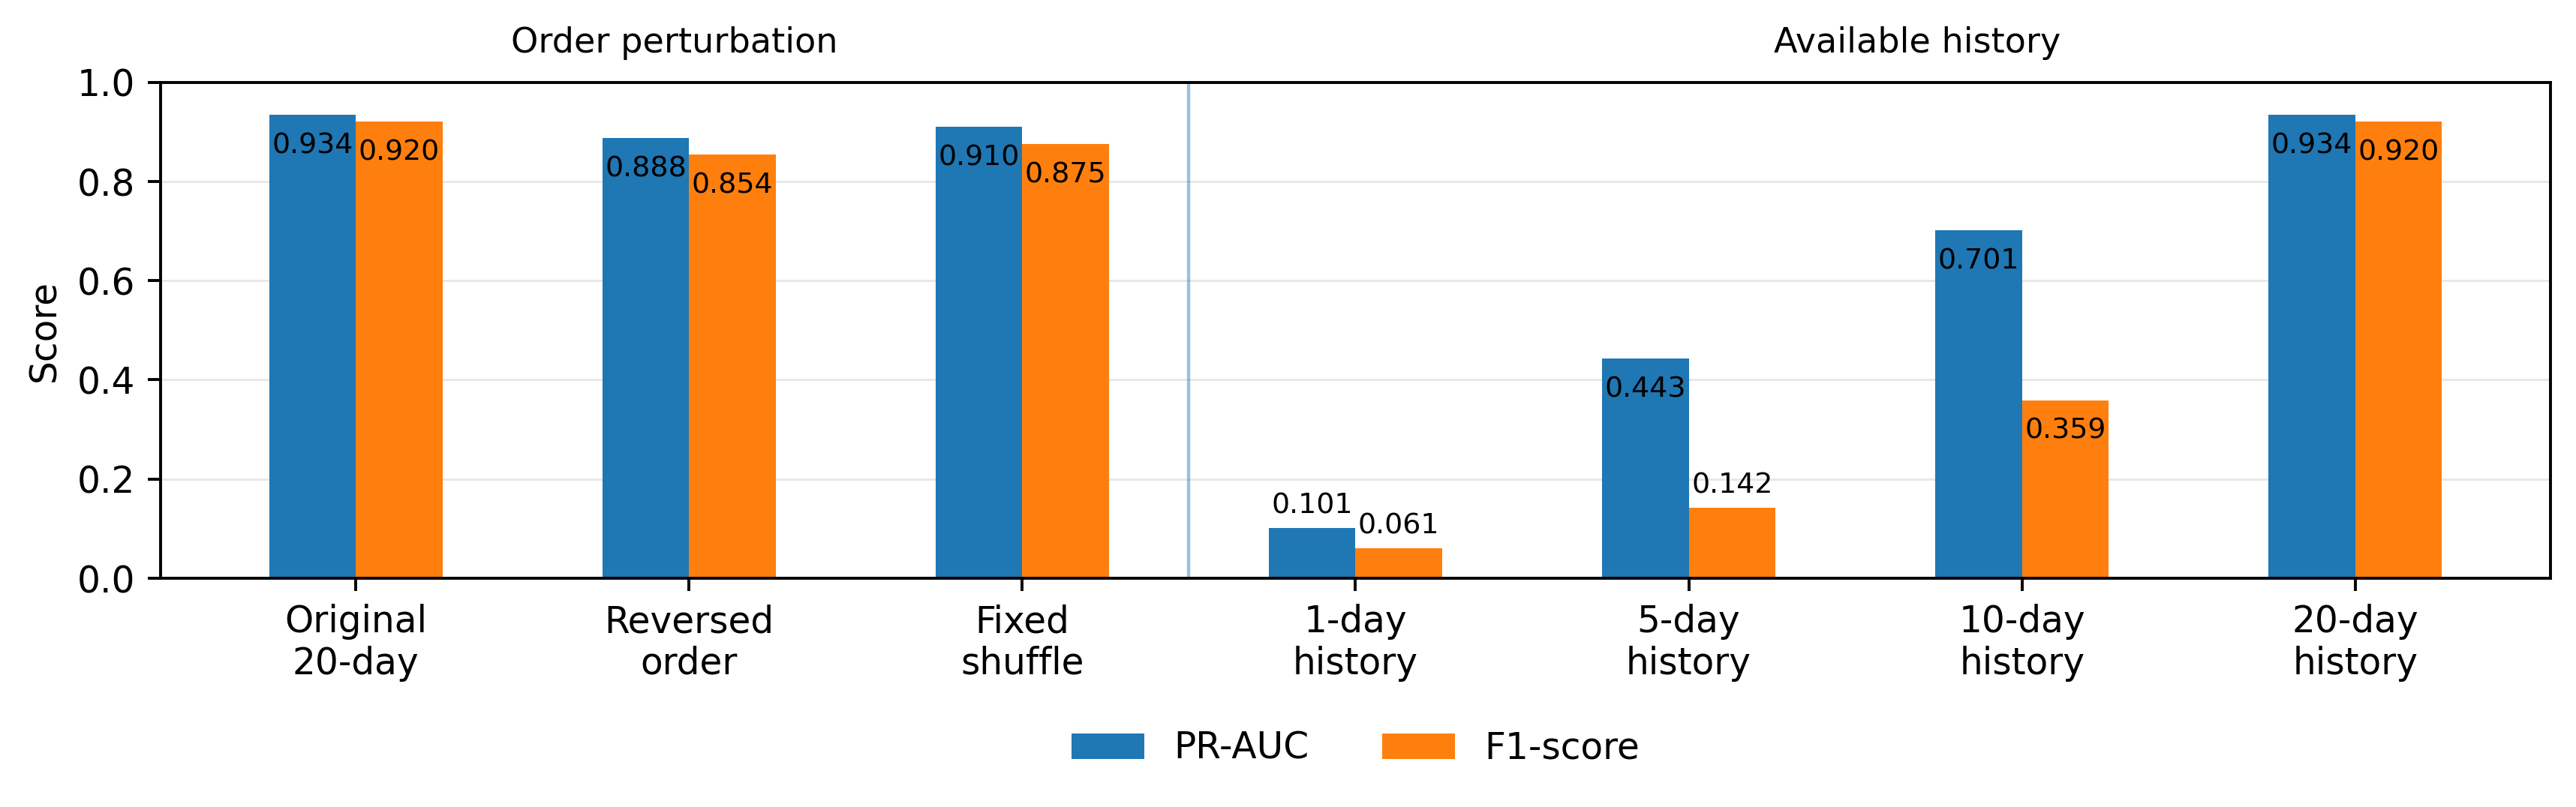
\includegraphics[width=\columnwidth,keepaspectratio]
{figures/fig_temporal_value_results.png}
\caption{Temporal-order and partial-history analysis. The first three
conditions perturb the order of the same observations; the remaining
conditions increase behavioural history from one to 20 days.}
\label{fig:r52_temporal_value_fig}
\end{figure}

% -----------------------------------------------------------------------------
% Structured explanation and degraded-input results
% -----------------------------------------------------------------------------
\subsection{Structured Explanation and Degraded-Input Results}
\label{subsec:explanation_results}
The explanation procedure was developed on CERT r4.2 and repeated using the
final CERT r5.2 teacher-anchored students. The analysis covered temporal
attention, original-input occlusion, ODST routes, reached leaves, individual
tree outputs, reference-centred tree contributions, source-channel
ablation, and Gaussian-noise sensitivity.

\smallskip
Temporal attention was first examined using twelve deterministically
selected CERT r4.2 validation cases. The sample contained three
true-positive, three true-negative, three false-positive, and three
false-negative cases. Figure~\ref{fig:temporal_attention_cases} shows one
deterministically selected case from each outcome category.

\begin{figure}[!tbp]
\centering
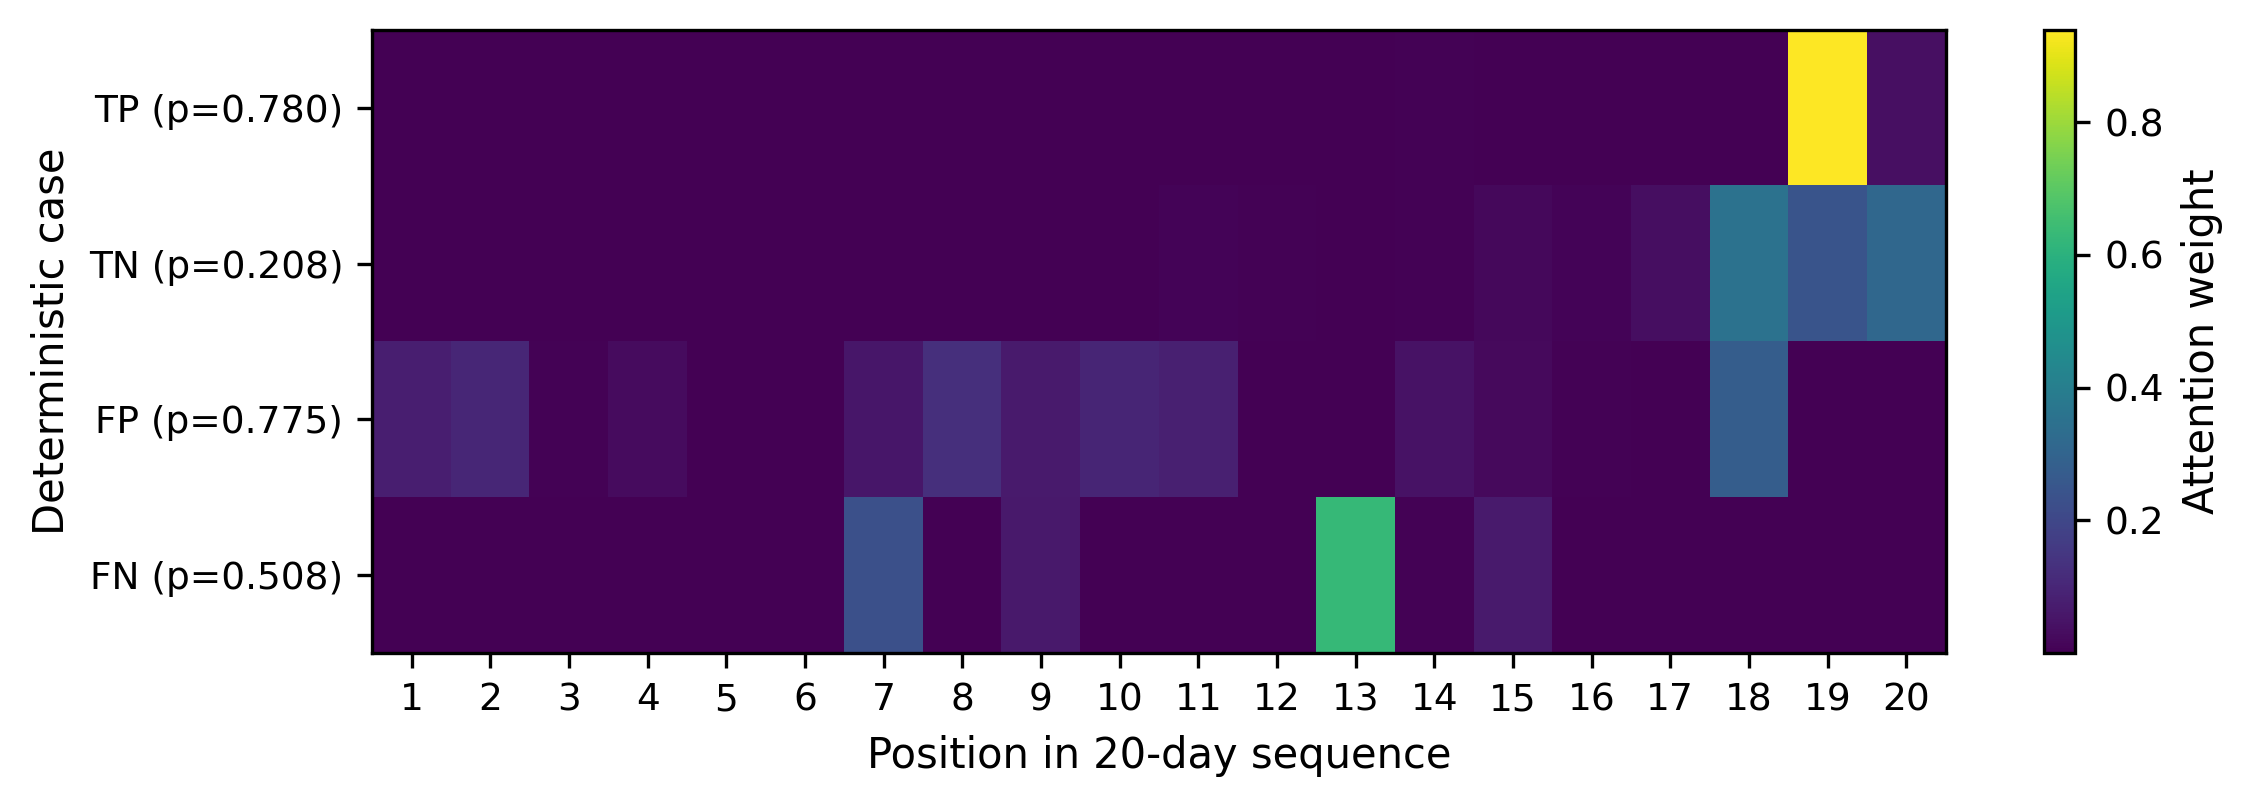
\includegraphics[
width=0.98\columnwidth,
keepaspectratio
]{figures/fig_teacher_temporal_cases.png}
\caption{Temporal attention across the 20-day input for deterministically
selected CERT r4.2 seed-42 true-positive, true-negative, false-positive,
and false-negative cases. Brighter cells indicate greater attention at the
corresponding sequence position.}
\label{fig:temporal_attention_cases}
\end{figure}

Each row in Figure~\ref{fig:temporal_attention_cases} represents one
prediction outcome, while the columns represent the 20 positions in the
behavioural sequence. The attention patterns concentrated on different
positions across the four cases. The true-positive case placed most
attention near the end of the sequence, whereas the false-negative case
concentrated more strongly on an earlier position. The figure therefore
shows which parts of the behavioural window received greater model
emphasis. Attention weights are interpreted as temporal evidence rather
than complete causal explanations.

\smallskip
The explanation mechanism was then evaluated on the final CERT r5.2
students through reference-centred tree contributions, attention fidelity,
original-input occlusion, source ablation, and Gaussian-noise sensitivity.
Table~\ref{tab:r52_explanation_portability} summarises the principal
findings.

\begin{table}[!tbp]
\caption{CERT r5.2 Explanation and Degraded-Input Evidence}
\label{tab:r52_explanation_portability}
\centering
\footnotesize
\renewcommand{\arraystretch}{1.08}
\setlength{\tabcolsep}{2pt}
\begin{tabularx}{\columnwidth}
{@{}>{\raggedright\arraybackslash}p{1.75cm}Y@{}}
\hline
\textbf{Dimension} &
\textbf{Completed result} \\
\hline
Centred ODST faithfulness &
Top-minus-random confidence intervals excluded zero for seeds 42, 52, and
62 at \(k=3,5,10\). The centred contributions reconstructed the ODST
readout exactly. \\
Attention fidelity &
Top-attention interventions produced positive comprehensiveness differences
relative to matched random positions across seeds and intervention sizes. \\
Original features &
For seed 42, \emph{has\_file\_activity} and
\emph{has\_device\_activity} produced the strongest occlusion effects. \\
Source ablation &
Removing file evidence produced the largest scaled-space effect, followed
by device evidence. \\
Noise and route stability &
Gaussian noise produced dose-dependent PR-AUC degradation. Route and leaf
agreement remained high at \(\epsilon=0.05\) when the predicted class was
unchanged. \\
\hline
\end{tabularx}
\end{table}

Figure~\ref{fig:odst_faithfulness_matrix} summarises the
reference-centred ODST faithfulness result across the final CERT r5.2 seeds
and intervention sizes.

\begin{figure}[!tbp]
\centering
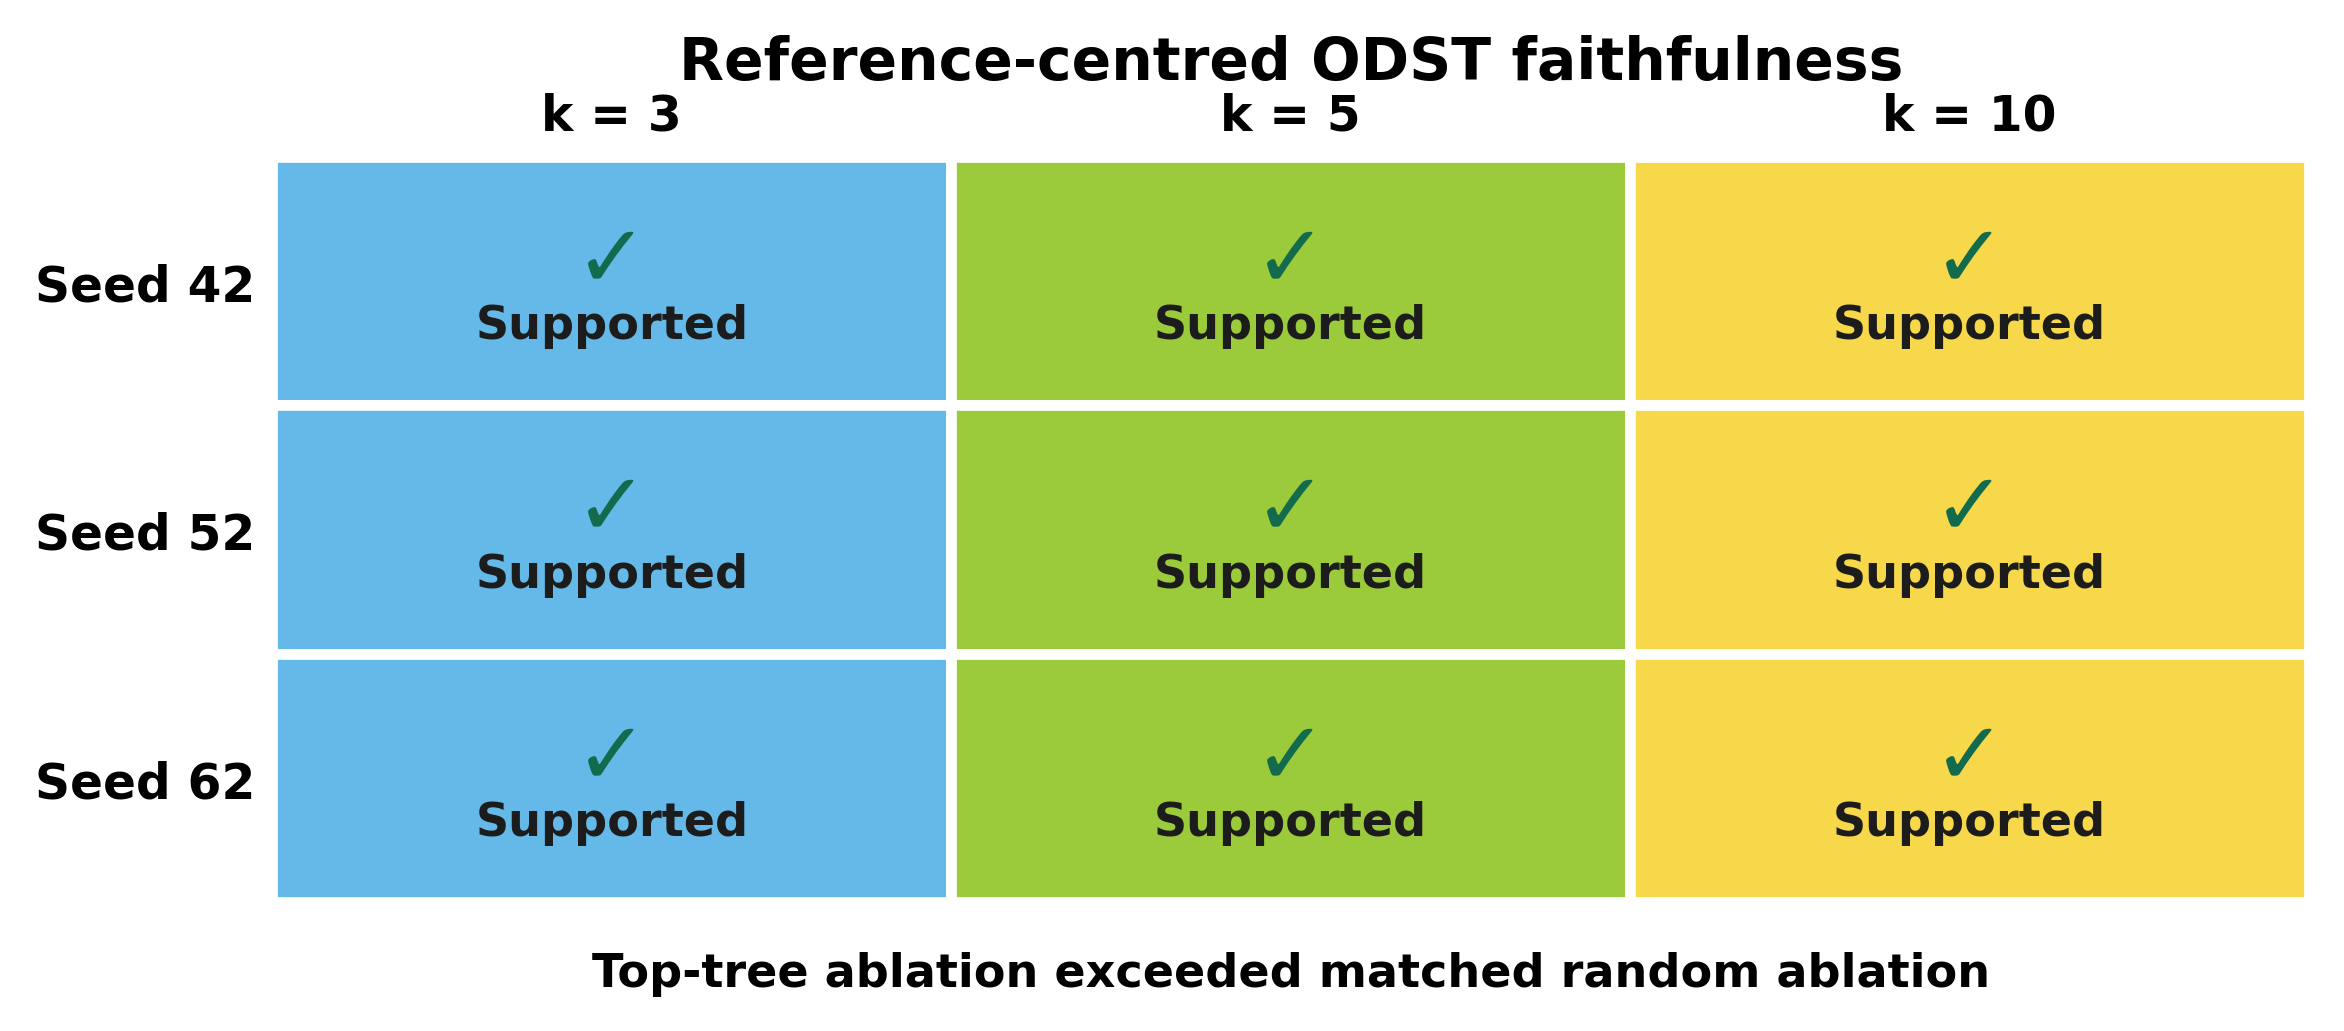
\includegraphics[
width=0.96\columnwidth,
keepaspectratio
]{figures/fig_odst_faithfulness_matrix.png}
\caption{Reference-centred ODST faithfulness across the final CERT r5.2
students. Every seed--\(k\) combination was supported, and the centred
contributions reconstructed the ODST readout exactly.}
\label{fig:odst_faithfulness_matrix}
\end{figure}

Reference-centred tree-contribution rankings were faithful under the defined
top-versus-random intervention across all three final CERT r5.2 seeds;
routes and reached leaves remained traceable internal outputs rather than
independently validated attributions. Removing the trees identified as most
influential changed the model output more than removing the same number of
randomly selected trees. Ranking by raw absolute tree output, together with
centred ranking against the median training reference, is retained
separately as a sensitivity analysis. A disclosed explanation-only post-hoc
analysis on the previously accessed CERT r5.2 test partition reproduced the
centred pattern and is used only as corroborating explanation evidence.

\smallskip
The explanation mechanism transferred across CERT versions, although the
most influential original features and source channels varied between the
datasets. This supports portability of the explanation procedure rather
than identical explanation content.

\smallskip
Source ablation and Gaussian noise quantified model dependencies and
continuous-input sensitivity under controlled degraded-input conditions.
These experiments are not adversarial evasion or training-time poisoning
evaluations.

% -----------------------------------------------------------------------------
% Calibration, alert burden, and computation
% -----------------------------------------------------------------------------
\subsection{Calibration, Alert Burden, and Computational Results}
\label{subsec:calibration_runtime_results}
Grouped out-of-fold temperature scaling improved ODST probability
calibration. Table~\ref{tab:r52_calibration_alert} reports the seed-42
calibration values and alert consolidation.

\begin{table}[!tbp]
\caption{Seed-42 ODST Calibration and Alert Consolidation}
\label{tab:r52_calibration_alert}
\centering
\footnotesize
\renewcommand{\arraystretch}{1.08}
\setlength{\tabcolsep}{2pt}
\begin{tabular*}{\columnwidth}
{@{\extracolsep{\fill}}lcc@{}}
\hline
\textbf{Item} &
\textbf{Uncalibrated} &
\textbf{Temperature-scaled} \\
\hline
Brier score & 0.175 & 0.004 \\
ECE & 0.413 & 0.005 \\
\hline
\multicolumn{3}{@{}l@{}}{\textit{Alert consolidation}} \\
Sequence alerts & \multicolumn{2}{c@{}}{661} \\
Unique alerted users & \multicolumn{2}{c@{}}{36} \\
One-day-gap episodes & \multicolumn{2}{c@{}}{42} \\
\hline
\end{tabular*}
\end{table}

\begin{table}[!t]
\caption{ODST Simplification and Batch-32 Latency}
\label{tab:odst_simplification_latency}
\centering
\footnotesize
\renewcommand{\arraystretch}{1.08}
\setlength{\tabcolsep}{0pt}
\begin{tabular*}{\columnwidth}
{@{\extracolsep{\fill}}lcccc@{}}
\hline
\textbf{Model} &
\shortstack{\textbf{Head}\\\textbf{parameters}} &
\shortstack{\textbf{Latency}\\\textbf{(ms)}} &
\shortstack{\textbf{PR-AUC}\\\textbf{change}} &
\shortstack{\textbf{F1}\\\textbf{change}} \\
\hline
16-tree model &
8,977 &
2.331 &
Reference &
Reference \\
8-tree ablation &
4,489 &
2.503 &
\(-0.0004\) &
\(-0.006\) \\
\hline
\end{tabular*}
\end{table}

Temperature scaling preserved ranking exactly within each fold. Because
each fold used its own fitted temperature, globally stitched out-of-fold
ranks were not interpreted as directly comparable. ODST and
attention--linear showed near-parity at the predefined alert budgets. The
42 one-day-gap episodes are analytical temporal groupings rather than
independently verified real-world incidents.

\smallskip
The eight-tree ablation examined whether a smaller ODST head could retain
its predictive and explanation properties while reducing runtime.
Table~\ref{tab:odst_simplification_latency} reports the result.

The eight-tree model halved the head parameter count and retained
reference-centred faithfulness, while PR-AUC and F1 changed only slightly.
Its batch-32 latency was nevertheless approximately 7.4\% higher (2.503
versus 2.331\,ms), so it did not satisfy the predefined efficiency
objective. The protected 16-tree configuration was retained.

\smallskip
Component-level profiling showed that the ODST head accounted for
approximately 72--73\% of device-resident inference latency. The complete
ODST model also required approximately 3.7 times the batch-32 latency of
attention--linear. These findings identify ODST execution, rather than
parameter count alone, as the main target for future runtime optimisation.

\smallskip
Overall, the results identify the Bi-LSTM--attention pathway as the
principal temporal predictive component, teacher anchoring as the
end-to-end optimisation contribution, ODST as the explanation-oriented
differentiable head, and attention--linear as the efficiency- and
raw-calibration-oriented neural reference. RF and XGBoost remain strong
engineered-tabular references under both the one-pass and same-information
protocols.